Here we present the specific choices we chose to incorporate into our system.  
%This section presents the implementation of our three step methodology presented in Section \ref{sec:multiscale-framework}.
%We start by describing the methods behind the initial state construction in Section \ref{sec:state-construction-impl}
%and then continue to present implementation details of steps two and three in sections \ref{sec:transition-probs-impl}
%and \ref{sec:state-aggregation-impl} respectively.
%%
%
%\subsection{Initial State Construction}
%\label{sec:state-construction-impl}
%
%As described in section \ref{sec:framework-states} 
The first step in the pipeline, which is the construction of the partition of the space and the initial (finest scale) Markov chain.
There are many partitioning/clustering algorithms in the literature, including many that produce a hierarchical partition.% Most depend on a distance matrix between the data points, leading to a computational complexity of $O(n^2)$, rendering 
 %them unsuitable for large datasets.
%Many of these algorithms construct a hierarchy which has $n$ levels,  
We opt to first construct a partition and then construct hierarchy. This is a design choice which decouples the choice of partition construction and the choice of aggregation strategy.  For larger datasets, this is also more computationally efficient, since after the initial partition is constructed, the complexity of constructing a partition is determined by the number of states in this partition rather than the number of data points.  	
%To avoid , we first create a flat partition of the data space and later aggregate these
%partitions to obtain a hierarchical structure.


%Following the intuition of Section \ref{sec:framework-states}
To construct the partition, two data points are considered similar if they lie close
to each other. We use Euclidean distance but any metric amy be used.
%
In StreamStory, we implemented $k$-means~\cite{Maimon:2005:DMK:1088958} and DP-means \cite{DBLP:journals/corr/abs-1111-0352} to construct the partition. Each  
partition  represents a  Voronoi cell around its centroid. 
%
% \primoz{When using StreamStory processes data in real time, the current state is thus selected by assigning the current sample to the nearest centroid using the following formula:
% \begin{equation}
% 	\nonumber
% 	i = \argmin_{i \in \mathbb{N}_k} \|x - \mu_i\|.
% \end{equation}
% This shoudl come later}
%
The number of centroids (in case of $k$-means) or the cluster radius (in case of DP-means) should
be chosen based on domain knowledge and the level of detail users desire. This parameter also effects the 
initial construction time, meaning for large datasets we may want to limit the number of states.

%\subsection{Modeling Transition Probabilities}
%\label{sec:transition-probs-impl}

%As described in Section \ref{sec:framework-transitions} we model state transitions using the continuous
%time Markov chain framework, first presented in Section \ref{sec:preliminaries}. 

Once the partition is computed, the new transition probabilities are computed using Equation~\ref{eq:ctmc-state-aggregation}.
%
The system enables users to select a subset of attributes which are used to model the transition rates. Since the
jump process in a Markov chain from state $i$ to state $j$ can be characterized as a Poisson process, we can model its
transition rate $q_{ij}$ as a function of these attributes $q_{ij} = q_{ij}(x)$. We do this by discretizing the continuous time parameter into a discrete sequence $(0, \epsilon, 2\epsilon, ...)$ and
estimate the transition rates as
\begin{equation}
	q_{ij}(x) = \frac{\epsilon}{\tilde{p}_{ij}(x)}
\end{equation}
where $\tilde{p}_{ij}(x)$ is the estimated probability of jumping from state $i$ to state $j$ in time
$\epsilon$.
%
Suppose the process is in state $i$ at time $t$ and define the random variable 
$$J_i = j \Leftrightarrow X_{t + \epsilon} = j.$$
$J_i$  has a multinomial distribution with parameters $(p_{i1}, p_{i2}, ..., p_{in})$ which can be 
modeled using a nominal logistic regression model~\cite{glm-introduction} to estimate $\tilde{p}_{ij}(x)$.
The transition rate matrix is then constructed from a matrix of logistic regression models -- one for each possible transition. 

Modeling and estimating the transitions in this way is computationally efficient and provides a basis for aggregation step described below. As we will show in our examples (Section~\ref{sec:experiments}), these provide an intuitive interpretation of the transitions helping us understand the dynamics. 	

% \lstopar{
% We need to explain why modeling transitions using signals is useful and why it is used.
% In previous documents I went on blabbering that by modeling transitions this way, we allow
% the possibility of users observing the dynamics in alternate configurations and simulating
% what would happen if they changed some parameter. (This was more or less BS though)
% }
Finally, to visualize the Markov chain, we use multi-dimensional scaling (MDS) \cite{} on the graph, where larger transition probabilities correspond to higher similarities. We then use an iterative repulsive scheme to ensure that the states do not overlap in the final visualization. 

\subsection{Aggregation}
\label{sec:state-aggregation-impl}

With the initial partition computed, we must construct the hierarchy by merging partitions. We previously assumed a merging function, i.e. $\phi$, was given. Here, we present two schemes for conmputing $\phi$: one based on agglomerative clustering~\cite{Murtagh83} and another based on the properties of the Markov chain. 

Agglomerative clustering represents each partition by its centroid. It computes a distance matrix $D \in \mathbb{R}^{n \times n}$ with each element $(D)_{ij}$ representing the distance between $c_i$ and $c_j$ (the $i$-th and $j$-th centroids respectively). This can be used with any metric, however in our examples we restrict oursleves to Euclidean distance.
%we follow the intuition from Section \ref{sec:framework-states} and use Euclidean distance between the state centroids:
\begin{equation}
	\nonumber
	(D)_{ij} = d(c_i, c_j) = \|c_i - c_j\|_2
\end{equation}
The algorithm then recursively merges pairs of clusters until only a single cluster remains, producing a cluster tree or \emph{dendrogram}. The partitions chosen for merging are the ones with the minimal entry in the distance matrix $D$:
\begin{equation}
	\nonumber
	(i_{min},j_{min}) = \argmin\limits_{i \neq j}(D)_{ij}.
\end{equation}
Once the clusters are merged, the entries in the distance matrix that correspond to the merged clusters are updated. This update is called the linkage criterion \cite{Hartigan:1975:CA:540298}. It determines the distance between clusters as a function of the pairwise distances between their elements. The most popular linkage criteria in the literature are: single-linkage, complete-linkage and average (or mean) linkage. Note that here the elements of clusters are centroids rather than the data points. 
Our initial experiments show no significant difference between the three and therefore we chose to use the mean linkage criterion:
\begin{equation}
	\nonumber
	D_{S_i,S_j} = \frac{1}{\left|S_i\right|\left|S_j\right|}\sum\limits_{i \in S_i}\sum\limits_{j \in S_j} d(c_i,c_j)
\end{equation}
The distance between the merged clusters $D_{i_{min} j_{min}}$ is used as the height of the resulting dendrogram, or in our case, as the scale where the merged state/cluster first appears. Therefore, each merge generates a new Markov chain (see Figure~\ref{fig:dendrogram}).% shows this relationship between the dendrogram and \lstopar{our visualization}.
\begin{figure}[h!]
	\centering
	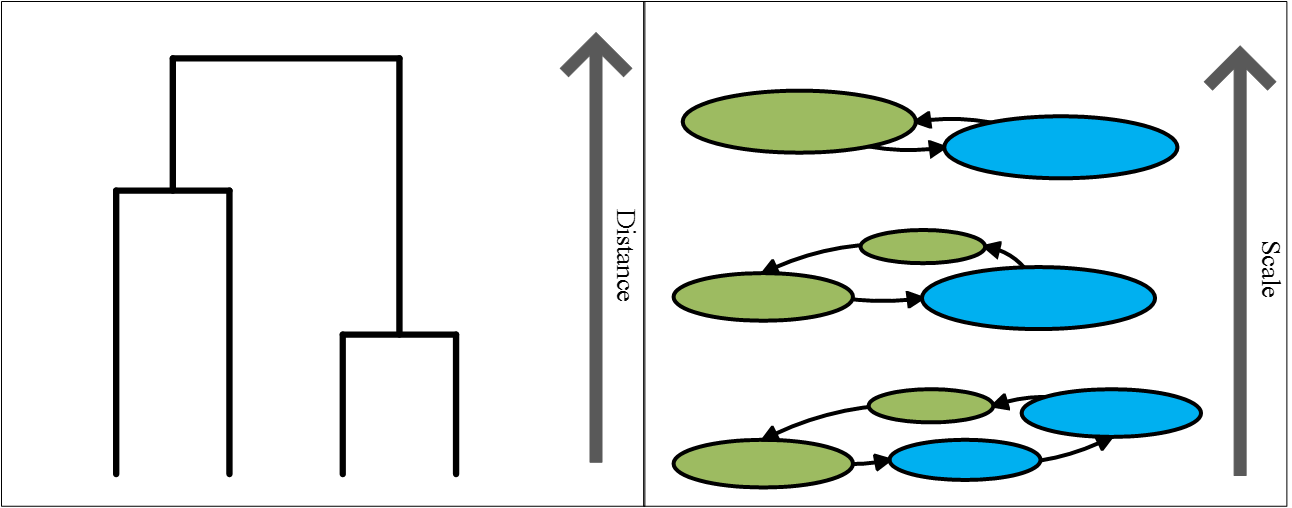
\includegraphics[width=\columnwidth]{dendrogram}
	\caption{The relationship between a dendrogram and \lstopar{scale}. The $y$-coordinate in a dendrogram represents the scale where the corresponding state appears in our \lstopar{visualization}.}
	\label{fig:dendrogram}
\end{figure}
%
To assign a scale value, the initial states are assigned the scale $0$. For coarser-scale, aggregated states, we compute the scale as follows. Let $S$ be a state constructed by aggregating states $A$ and $B$.  The scale of $S$ is then defined as:
\begin{equation}
	\nonumber
	s(S) = \frac{1}{\left|A\right|\left|B\right|}\sum\limits_{i \in A}\sum\limits_{j \in B} d(c_i,c_j)
\end{equation}
Intuitively in this case, the scale provides a measure of distance between individual states inside an aggregated, higher level state.


The second aggregation method we propose is an extension of the algorithm proposed in \lstopar{[TODO cite]} to continuous time Markov chains and represents a top-down approach. Beginning with our initial Markov chain, we initially assign all the states into a single state. This represents the coarsest possible scale. We then split this state into two by approximating the \emph{min-cut} problem in the graph representing the Markov chain. 

The method then works iteratively, splitting the ``best" partition until we have the initial Markov chain.
%
The splitting procedure is based on spectral bi-partitioning of Markov chains using the sign-structure of the eigenvector, corresponding to the second largest eigenvalue of the \emph{symmetrized transition rate matrix} $Q_s$. Indeed,  the transition rate matrix of a continuous time Markov chain $Q$ is exactly the negative Laplacian of the corresponding directed weighted graph~\cite{Agaev2005157}.
%
$Q$ in general will not be symmetric and so may have complex eigenvalues. We therefore first symmetrize $Q$,
\begin{equation}
	\nonumber
	Q_s = \frac{1}{2}(\Pi Q + Q' \Pi)
\end{equation}
where $Q_s$ is \emph{symmetrized version} of $Q$ and $\Pi = diag(\pi)$ is a diagonal matrix with the stationary distribution on the diagonal. This ensures that all the eigenvalues (and eigenvectors) are real-valued and furthermore matrix $\pi^{-1}Q_s$ preserves the ergodic properties of $Q$. 

The bi-partition function $\phi: I \rightarrow \{0,1\}$ is obtained by solving the following generalized eigenvalue problem:
\begin{equation}
	Q_s v = \lambda_2 \Pi v.
\end{equation}
and assigning states based on the sign structure of $v$:
\begin{equation}
	\nonumber
	\phi(i) = 
		\left\{
			\begin{array}{ll}
				1 & \mbox{if } v_i \ge 0 \\
				0 & \mbox{otherwise}
			\end{array}
		\right.
\end{equation}

 The iterative algorithm begins by assigning  all the states of the original Markov chain to a single state. On the $m$-th iteration, it assumes that $m$ splits have already occured and selects which of the $m$ partitions to further split. 

 Let $Q^{(i)}$ be a transition rate matrix of the Markov chain induced on the states in the $i$-th partition. Bi-partitioning $Q^{(i)}$ then provides $m+1$ partitions which induce a Markov chain on $m+1$ states with a transition rate matrix $Q_{m+1}^{(i)}$ computed using Equation~\ref{eq:ctmc-state-aggregation}. The algorithm selects which of the $m$ partitions to split by minimizing the relative entropy rate between $Q$ and $Q_{m+1}^{(i)}$:
\begin{equation}
	i = \argmin\limits_{i \in \mathbb{N}_m} D(Q || Q_{m+1}^{(i)}).
\end{equation}
The relative entropy rate $D(Q || Q_{m+1}^{(i)})$ provides a measure of ``distance" between the aggregated Markov chain and the original. When two Markov chains $Q$ and $\tilde{Q}$ are defined on the same state space $I$, the relative entropy rate between the two is defined as \cite{EJP374}:
\begin{equation}
	\label{eq:relative-entropy-rate}
	D(Q || \tilde{Q}) = \sum\limits_{\substack{i,j \in I \\ i \neq j}}\pi_i q_{ij} \log\frac{q_{ij}}{\tilde{q}_{ij}} + \sum\limits_{i \in I}\pi_i(q_{ii} - \tilde{q}_{ii})
\end{equation}
Since $Q$ and $Q_{m+1}^{(i)}$ are not defined on the same state space, we cannot use Equation~\ref{eq:relative-entropy-rate} directly. Let $\phi_s: I \rightarrow J$ denote the partition function, mapping states of $Q$ into states of $Q_{m+1}^{(i)}$ and let $\psi = \phi \circ \phi^{-1}$. Therefore, $\psi(i) \subseteq I$  represents the set of states which were aggregated into a single state in $\phi(i) \in J$. We now define $q_{i\psi(j)} = \sum_{k \in \psi(j)}q_{ik}$ and $\tilde{q}_{kl} = \left(Q_{m+1}^{(i)}\right)_{kl}$. Using this notation, we can define the relative entropy between $Q$ and $Q_{m+1}^{(i)}$ as:
\begin{equation}
	D(Q || Q_{m+1}^{(i)}) = \sum\limits_{\substack{i,j \in I \\ \phi(i) \neq \phi(j)}}\pi_i q_{ij}\log\frac{q_{i\psi(j)}}{\tilde{q}_{\phi(i)\phi(j)}} + \sum\limits_{i \in I}\pi_i \left(q_{i\psi(i)} - \tilde{q}_{\phi(i)\phi(i)}\right).
\end{equation}
%
%We refer the reader to \lstopar{Appendix A} for more details.
\noindent \paragraph{\bf Computing the multiscale layout:}
To visualize the different scales, we use the MDS coordinates computed at the initial level. When states are aggregated, the position of the new state is computed as the weighted average of the states' positions. As with the initial layout, this is followed by a repulsive scheme to ensure that the states do not overlap.

%\lstopar{I'll check if the weights are based on the number of states aggregated or on the stationary distribution.}

